\documentclass[12pt,fleqn]{article}
\usepackage{
    amsfonts,
    amsmath,
    amssymb,
    amsthm,
    booktabs,
    enumerate,
    flexisym,
    graphicx,
    setspace,
    slantsc,
    tabularx,
    url,
}

\title{Smooth interpolation for Impulse Response Functions from \allcaps{svar}s}
\author{Gray Calhoun}
\date{2015-03-27}
% The LaTeX macros in this file are available through the CC0 license
% (creative commons public domain.  See
% <http://creativecommons.org/publicdomain/zero/1.0> for more
% details.)  To the extent possible under law, the copyright holders
% have waived all copyright and related or neighboring rights to the
% contents of this file.

\usepackage[letterspace=35]{microtype}
\newcommand{\allcaps}[1]{\textls{\MakeUppercase{#1}}}

\newcommand{\AIC}{\allcaps{AIC}}
\newcommand{\BIC}{\allcaps{BIC}}
\newcommand{\BRC}{\allcaps{BRC}}
\newcommand{\CDF}{\allcaps{CDF}}
\newcommand{\CLT}{\allcaps{CLT}}
\newcommand{\DGP}{\allcaps{DGP}}
\newcommand{\FCLT}{\allcaps{FCLT}}
\newcommand{\FWE}{\allcaps{FWE}}
\newcommand{\GDP}{\allcaps{GDP}}
\newcommand{\HAC}{\allcaps{HAC}}
\newcommand{\IRF}{\allcaps{IRF}}
\newcommand{\IRFs}{\allcaps{IRF}s}
\newcommand{\LLN}{\allcaps{LLN}}
\newcommand{\LM}{\allcaps{LM}}
\newcommand{\MA}{\allcaps{MA}}
\newcommand{\MDS}{\allcaps{MDS}}
\newcommand{\MSE}{\allcaps{MSE}}
\newcommand{\NBER}{\allcaps{NBER}}
\newcommand{\NSF}{\allcaps{NSF}}
\newcommand{\NED}{\allcaps{NED}}
\newcommand{\OLS}{\allcaps{OLS}}
\newcommand{\OOS}{\allcaps{OOS}}
\newcommand{\SFWE}{\allcaps{SFWE}}
\newcommand{\SPA}{\allcaps{SPA}}
\newcommand{\VAR}{\allcaps{VAR}}
\newcommand{\WFWE}{\allcaps{WFWE}}


\urlstyle{same}
\newcolumntype{C}{>{\centering\arraybackslash}X}

\usepackage[small]{caption}
\usepackage[T1]{fontenc}
\usepackage[margin=1.25in]{geometry}
\usepackage[charter]{mathdesign}
\usepackage[letterspace=35]{microtype}
\usepackage[sort,round,comma]{natbib}
\bibliographystyle{abbrvnat}
\newcommand\citepos[2][]{\citeauthor{#2}'s \citeyearpar[#1]{#2}}
\newcommand\poscw{\citeauthor{ClW:06}'s \citeyearpar{ClW:06,ClW:07}}
\newcommand\citen[1]{\citeauthor{#1}, \citeyear{#1}}

\renewcommand{\Re}{\operatorname{Re}}
\renewcommand{\Im}{\operatorname{Im}}

\DeclareMathOperator{\whitenoise}{\mathit{white\ noise}}
\newcommand{\vep}{\varepsilon}
\newcommand{\AR}{\allcaps{AR}}
\newcommand{\RR}{\mathbb{R}}

\begin{document}
\maketitle

Impulse Response Functions (\IRF s) are used in signal processing and
time-series analysis to represent the effect over time of a short
impulse or shock on a dynamic system; and they are heavily used in
Macroeconomics to characterize the effects of a shock of theoretical
interest --- the effect of a monetary policy shock, for example, or a
technology shock. Formally, if $y_t$ is a stochastic process with the
\MA($\infty$) representation
\begin{equation*}
  y_t = \sum_{j=0}^{\infty} \psi_j \vep_{t-j}
\end{equation*}
and $\vep_t \sim \whitenoise(0,\Sigma)$ where $\Sigma$ is normalized
to have diagonal elements equal to 1, the \IRF\ is the function
\begin{equation}\label{eq:1}
  \Psi(j) = \theta_j u
\end{equation}
for $j = 0, 1, 2,\dots$ where the vector $u$ has norm 1 and represents
a specific theoretical shock of interest. In Macroeconomics,
researchers usually don't work with \MA\ representations directly, but
instead model the processes as a finite lag \VAR, but the principle is
exactly the same.

An advantage of using \IRF s is that they show the full set of
dynamics implied by a particular parameter estimate of the \VAR, and
to make these dynamics more clear the values determined by
Equation~\eqref{eq:1} are typicially plotted as a graph and joined by
straight lines --- see the left column of Figure~\ref{f1} for several
examples. Indeed, these graphs and connecting lines are indespensible
when several \IRF s are plotted in the same graph to represent
statistical uncertainty or a set of potential dynamics --- without
some method of connecting the points, we can see the marginal
distributions of each estimate of $\Psi(j)$, but can not see their
joint distributions.

Unfortunately, the ubiquitous method of connecting the points
$\Psi(0), \Psi(1),\dots$, i.e.\ drawing a straight line between them,
can introduce misleading visual distortions, which we will explicitly
discuss later. In this paper, we show how the \IRF\ $\Psi(j)$ can be
meaningfully defined for \VAR s for any real positive value of $j$ and
give a convenient method for calculating it. (Figures~\ref{f1}
and~\ref{f2} have examples if you're impatient to see them.) This
allows researchers to use the estimated \VAR\ itself to interpolate
between the points for which it is usually defined and results in
graphs that do not have the distortions produced by linear
interpolation. Moreover, using the smoothed \IRF\ also allows for
refinements to partial identification strategies based on sign
restrictions.

\section{Motivation and results}

It is well known that any \VAR($p$) has a \VAR(1) ``canonical''
representation. If
\[
y_t = \sum_{i=1}^p A_i y_{t-i} + \vep_t
\]
then
\[
\begin{pmatrix}
  y_t \\ y_{t-1} \\ y_{t-2} \\ \vdots \\ y_{t-p+1}
\end{pmatrix}
=
\begin{pmatrix}
  A_1 & A_2 & \cdots & A_{p-1} & A_p \\
  I_k & 0   & \cdots & 0 & 0 \\
  0  & I_k  & \cdots & 0 & 0 \\
  \vdots & \vdots & & \vdots & \vdots \\
  0 & 0 & \cdots & I_k & 0 
\end{pmatrix}
\begin{pmatrix}
  y_{t-1} \\ y_{t-2} \\ y_{t-3} \\ \vdots \\ y_{t-p}
\end{pmatrix}
+
\begin{pmatrix}
  \vep_{t} \\ 0 \\ 0 \\ \vdots \\ 0
\end{pmatrix}
\]
or
\[
z_t = B z_{t-1} + v_t.
\]
This representation is convenient, because we have
\[
E_t z_{t+k} = B^k z_{t}
\]
for any integer $k$, so it is easy to recursively generate \IRF s.

Our proposal in this paper is to extend this to non-integer values of
$k$, by using
\[
E_t z_{t+k} = \Re(B^k) z_{t} = \Re(V D^k V^{-1}) z_t
\]
where $\Re(z)$ returns the real part of the complex number $z$. The
matrix $V$ is the matrix of eigenvectors of $B$ and the matrix $D$ is
a diagonal matrix containing the eigenvalues of $B$. When $k$ is an
integer, this product is guaranteed to be real, but it may be complex
in general.

Dropping the imaginary part works, because if $a_t$ is any real
sequence that satisfies $B a_{t-1} = a_t$ for the real matrix $B$,
then $a_t' = \Re(B^t) a_{0} \equiv \Re(V D^t V^{-1}) a_0$ trivially
satisfies the same recurrence relationship. Since $B$ is real, $B
\Re(B^{t-1}) = \Re(B^t)$ and we have
\begin{align*}
B a'_{t-1} &= B \Re(B^{t-1}) a_{0} \\
&= \Re(B^t) a_0 \\
&= a'_t.
\end{align*}

\section{Numerical example}

For a numerical example, consider the two-variable \VAR(2)
\begin{equation}
  \begin{pmatrix}
    y_{1t} \\ y_{2t}
  \end{pmatrix}
  =
  \begin{pmatrix}
    - 0.5 & 0.01 \\ 0.3 & 0.1
  \end{pmatrix}
  \begin{pmatrix}
    y_{1,t-1} \\ y_{2,t-1}
  \end{pmatrix}
  +
  \begin{pmatrix}
    -0.2 & 0.1 \\ -0.1 & 0.0
  \end{pmatrix}
  \begin{pmatrix}
    y_{1,t-2} \\ y_{2,t-2}
  \end{pmatrix}
  +
  \begin{pmatrix}
    \vep_{1t} \\ \vep_{2t}
  \end{pmatrix}
\end{equation}
and assume for the sake of argument that $(\vep_{1t},\vep_{2t}) \sim
N(0,I)$ represents the shocks of interest.

As described above, we will define the smooth \IRF s for a shock to
the first element as
\begin{equation*}
  \begin{pmatrix}
    \hat y_{1j} \\ \hat y_{2j}
  \end{pmatrix}
  =
  \begin{pmatrix}
    1 & 0 & 0 & 0 \\ 0 & 1 & 0 & 0
  \end{pmatrix}
  V D^j V^{-1}
  \begin{pmatrix}
    1 \\ 0 \\ 0 \\ 0
  \end{pmatrix}
\end{equation*}
with
\begin{equation}
V = \begin{pmatrix}
     0.23 + 0.30 i & 0.23 - 0.30 i  & 0.06 + 0.03 i & 0.06 - 0.03 i \\
     0.27 + 0.06 i & 0.27 - 0.06 i  & 0.12 + 0.13 i & 0.12 - 0.13 i \\
     0.71 + 0.00 i & 0.71 + 0.00 i  & 0.31 - 0.12 i & 0.31 + 0.12 i \\
    -0.23 - 0.47 i & -0.23 + 0.47 i & 0.92 + 0.00 i & 0.92 + 0.00 i
  \end{pmatrix}
\end{equation}
and
\begin{equation}
  D = diag(-0.33 + 0.42 i, -0.33 - 0.42 i, 0.13 + 0.14 i, 0.13 - 0.14 i)
\end{equation}
the matrices of eigenvectors and eigenvalues of
\begin{equation*}
  \begin{pmatrix}
   -0.5            &  0.01          & -0.2          & 0.1          \\
    0.3            &  0.1           & -0.1          & 0.0          \\
    1.0            &  0.0           &  0.0          & 0.0          \\
    0.0            &  1.0           &  0.0          & 0.0
  \end{pmatrix}.
\end{equation*}
The same equations hold for the \IRF s for a shock to the second
element of $y_t$, but now the last vector should be $(0, 1, 0, 0)'$.

\begin{figure}[t]
  \centering
  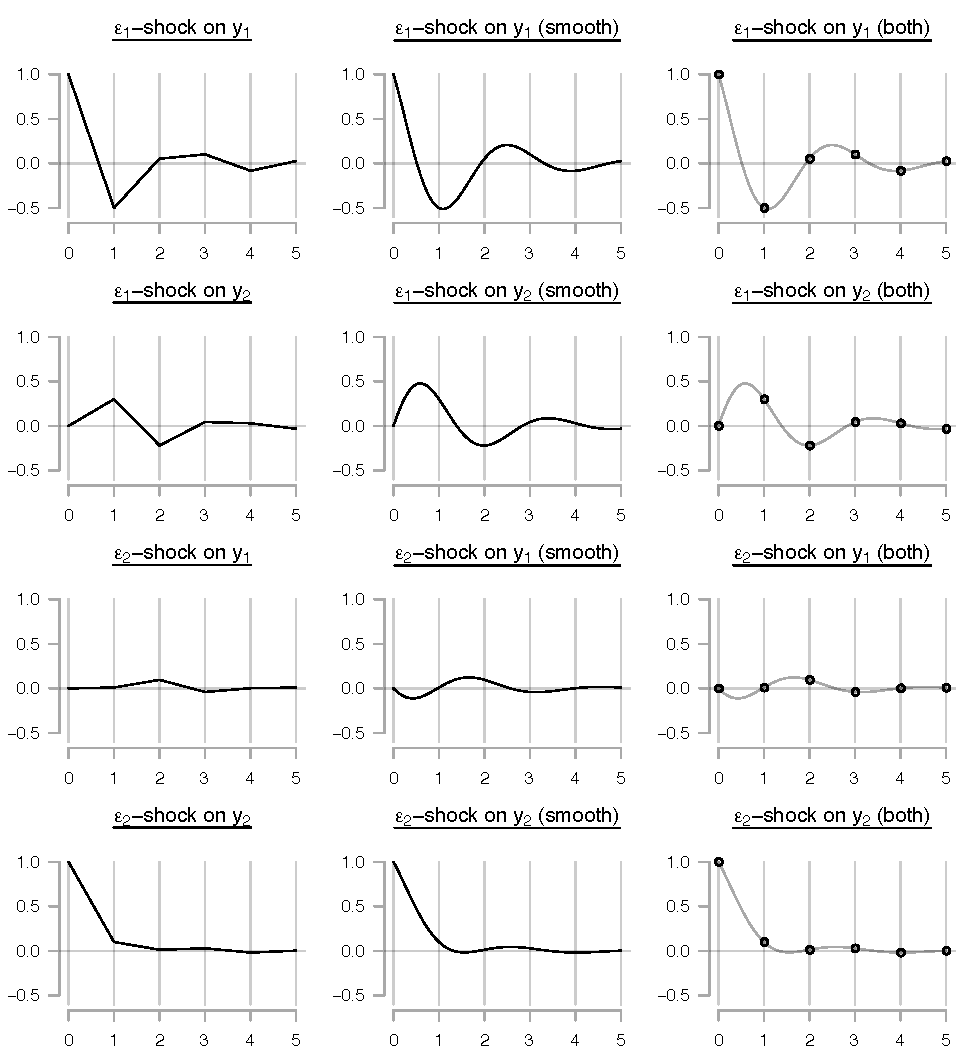
\includegraphics{graphs/numeric.pdf}
  \caption{Impulse Response Functions from example}
  \label{f1}
\end{figure}

We plot the \IRF s in Figure~\ref{f1}. The first column plots the
standard \IRF s and the second plots our proposed smooth
plots. Although the general impressions from both graphs are similar,
there are important differences. First, peaks and troughs are often
underestimated by the standard IRFs and their timing is frequently
misidentified. This is especially apparent in the first peak in the
second row. Second, even the sign of the \IRF\ can be misidentified,
as we see with the immediate response of $y_{1t}$ to a shock in
$y_{2t}$. Finally, unless turning points in the smooth functions
happen to coincide with integer values, discretizing the \IRF s
introduces misleading asymmetries and kinks.

\begin{figure}[t]
  \centering
  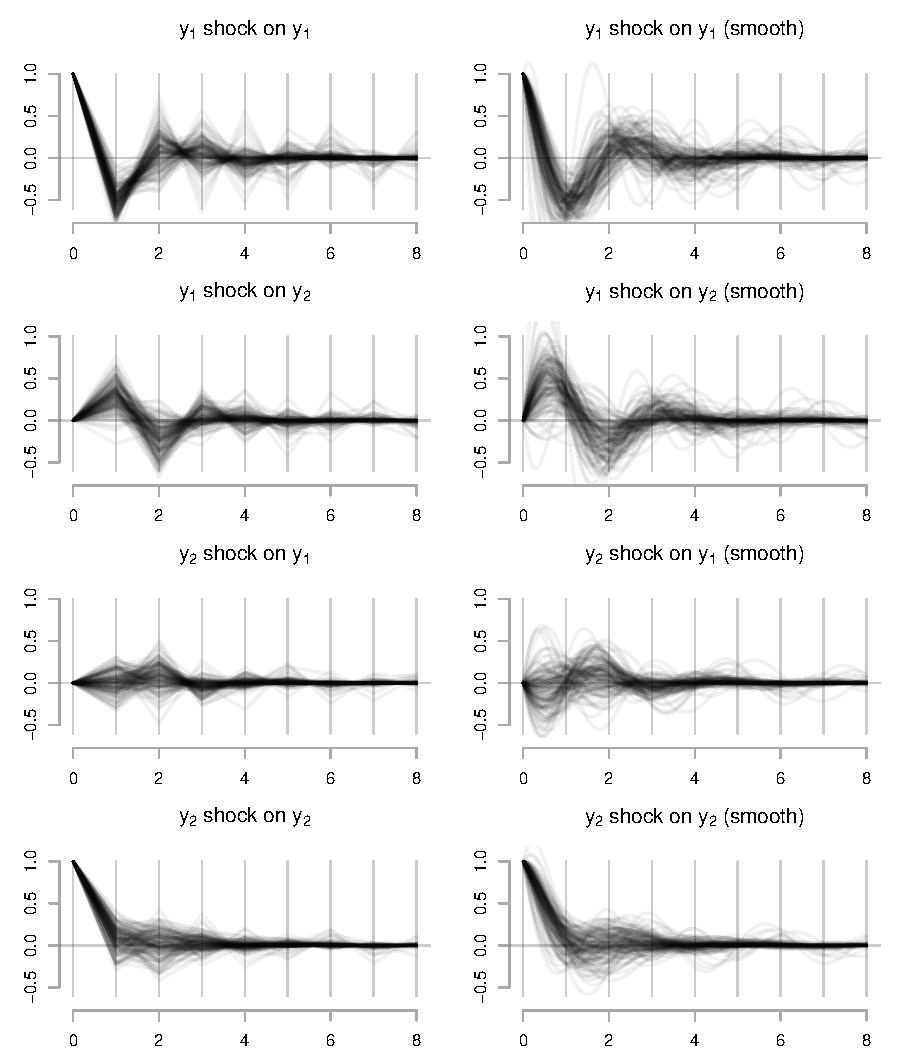
\includegraphics{graphs/numeric2.pdf}
  \caption{Impulse Response Functions from example}
  \label{f2}
\end{figure}

These distortions are even more apparent when we graph multiple
perterbations of the \IRF s in the same panel, which is a common way
of representing uncertainty or set-identified responses. To
demonstrate this phenomenon, we generated 150 replications of the \IRF
s by adding independent N(0, 0.15) noise terms to each element of $A$,
and then plotting the implied \IRF s as before.

These graphs are shown in Figure~\ref{f2}. The same issues apparent in
Figure~\ref{f1} are present here as well. But there are other problems
as well. In the first curve, for example, the discrete \IRF\ shows
that there is substantial negative correlation between the period 2
and period 3 estimated response and the period 3 and 4 response. But
the smoothed graph makes it clear that this is driven by the timing
and size of the first peak. When that peak is near period 2, the curve
has time to fall noticably before period 2, but when the peak is
closer to period 3, the curve is still rising for that interval. The
actual dynamics implied by the different curves are very
similar. Similar but less dramatic distortions appear in the other
panels as well. In the third row, for example, the discrete \IRF\
shows that about half of the parameter values have an initial increase
in response to a $y_{20}$ shock and half have an initial decrease, but
the smooth curves show that virtually all of them have an immediate
decrease, but that many start to increase very soon. The exact
location of the peak that falls between periods 1 and 2 determines
most of the initial dynamics, but this is impossible to see in the
discrete curve.

\section{Discussion}

Vector Autoregressive models do not just have implications for the
period-to-period dynamics of a stochastic process, they also have
implications about the very short-run dynamics within periods. In this
paper, we propose that researchers graph those intra-period dynamics
when plotting \IRF s and we give a simple method to do so, based on
the \VAR's canonical \VAR(1) representation. Even when researchers do
not want to assign any economic importance to these ultra short-run
dynamics, plotting them in the \IRF s minimizes visual distortions
that can arise from discretizing the dynamics, especially when several
\IRF s are plotted over eachother to represent uncertainty or set
identification --- see Figure~\ref{f2} for an example. If researchers
are willing to interpret these ultra short-run dynamics as having an
economic interpretation, they can also be used to refine sign
restrictions used in partial identification.

\end{document}
